\documentclass[aspectratio=169]{beamer}

\usepackage[english]{babel}
\usepackage{graphicx}
\usepackage{booktabs}
\usepackage{multirow}
\usepackage{amsmath, amsfonts, mathtools}
\usepackage{array}
\usepackage{pgfplots}
\pgfplotsset{compat=1.18}

\setbeamertemplate{navigation symbols}{}
\IfFileExists{beamerthemeTUDelft.sty}{%
  \usetheme{TUDelft}%
}{%
  \IfFileExists{beamerthemetud.sty}{%
    \usetheme{tud}%
  }{%
    \usetheme{Madrid}%
  }%
}

\title[Scenario 1 Progress]{Shared E-Scooter Rebalancing Simulation and RL Refinement\\Scenario 1 Progress Update}
\author[Y. Pan]{Yumeng Pan\\[0.4em]\small Supervisors: Dr. Shadi Sharif Azadeh, Dr. Yousef Maknoon\\Advisors: Jingyi (Rina) Cheng, Sara Momen}
\institute[TU Delft]{Delft University of Technology\\Faculty of Civil Engineering and Geosciences}
\date{\today}

\newcommand{\tightlist}{\setlength{\itemsep}{4pt}\setlength{\parskip}{0pt}}
\newcommand{\ph}[1]{\textcolor{gray}{\textit{#1}}}

\begin{document}

\begin{frame}
  \titlepage
\end{frame}

\begin{frame}{Agenda}
\begin{itemize}\tightlist
  \item Project scope and current boundary
  \item Implemented architecture and pipeline
  \item Scenario 1 design: behavior, reward, and RL setup
  \item Current progress and preliminary status
  \item Open issues and next steps
\end{itemize}
\end{frame}

\begin{frame}{Scope and Boundary}
\begin{columns}[T,onlytextwidth]
\begin{column}{0.48\textwidth}
\begin{block}{In Scope (Current Stage)}
\begin{itemize}\tightlist
  \item Event-driven simulation environment
  \item Zone/fleet/battery state transition
  \item OR output injection via \texttt{u\_odit.csv}
  \item User behavior simulation and KPI logging
  \item Scenario 1 RL refinement (DDQN)
\end{itemize}
\end{block}
\end{column}
\begin{column}{0.48\textwidth}
\begin{alertblock}{Out of Scope (Now)}
\begin{itemize}\tightlist
  \item OR optimization model redesign
  \item Scenario 2 implementation and analysis
  \item Final policy tuning and full ablation matrix
\end{itemize}
\end{alertblock}
\end{column}
\end{columns}
\end{frame}

\begin{frame}{System Architecture (Implemented)}
\begin{center}
\small
Trip Generator $\rightarrow$ Simulation Engine $\rightarrow$ OR Interface $\rightarrow$\\
User Choice $\rightarrow$ State Update $\rightarrow$ Metrics \\
\vspace{0.8em}
\normalsize
RL hook is inserted at OR-matched trip events (Scenario 1).
\end{center}

\vspace{0.8em}
\begin{block}{Key Design Principle}
Environment dynamics are independent from decision logic, so OR-only and OR+RL are directly comparable under aligned settings.
\end{block}
\end{frame}

\begin{frame}{Data and Execution Pipeline}
\begin{enumerate}\tightlist
  \item Run Sara OR model and export incentive plan
  \item Translate OR output to \texttt{u\_odit.csv}
  \item Build trip stream in simulator (current: stochastic generation)
  \item Execute simulation with OR-only or OR+RL mode
  \item Log transitions, reward decomposition, and KPI summaries
\end{enumerate}

\vspace{0.6em}
\begin{exampleblock}{Alignment Rule}
OR side and simulation side are connected only through the predefined interface file and shared time-window setup.
\end{exampleblock}
\end{frame}

\begin{frame}{Scenario 1: Decision and Behavior Logic}
\begin{block}{RL Action Space}
Binary decision at each OR opportunity: \texttt{offer} vs \texttt{no\_offer}.
\end{block}

\begin{block}{User Behavior (Single-layer Choice)}
\begin{itemize}\tightlist
  \item If offer exists: choose among \{offer, base, opt-out\}
  \item If no offer: choose among \{base, opt-out\}
  \item Choice is sampled from real-time utility-based probabilities
\end{itemize}
\end{block}

\begin{alertblock}{Scenario Assumption}
Scenario 1 keeps highest-battery-first scooter assignment logic unchanged.
\end{alertblock}
\end{frame}

\begin{frame}{Trip Generation in Simulation}
\begin{block}{Data Source and Interface}
\begin{itemize}\tightlist
  \item Trip requests are generated from aggregated OD demand profile (\texttt{omega\_od})
  \item OR side is unchanged; simulator reads OR decisions via \texttt{u\_odit.csv}
\end{itemize}
\end{block}

\begin{block}{Arrival Process (Current)}
\begin{itemize}\tightlist
  \item Distribution: NB2 (Negative Binomial) instead of Poisson
  \item Mean: from OD profile after scaling
  \item Dispersion: $\phi$ from hourly profile (\texttt{nb\_phi\_profile.csv})
\end{itemize}
\end{block}

\begin{alertblock}{Scaling Parameters}
\texttt{omega\_global\_scale}, \texttt{omega\_window\_scale}, \texttt{omega\_od\_target\_scale}
control trip density and offer-hit opportunity.
\end{alertblock}
\end{frame}

\begin{frame}{Training Workflow (Scenario 1)}
\begin{enumerate}\tightlist
  \item Run Sara OR model on fixed horizon and export incentive plan
  \item Translate OR output to \texttt{u\_odit.csv}
  \item Build 2-hour episodes with stochastic trip arrivals (NB2)
  \item At each OR-matched opportunity, RL selects \texttt{offer}/\texttt{no\_offer}
  \item Environment returns delayed transition and reward decomposition
  \item DDQN updates policy using replay buffer and target network
  \item Save checkpoints and evaluate OR-only vs OR+RL on aligned settings
\end{enumerate}

\vspace{0.4em}
\begin{exampleblock}{Core Principle}
RL is an execution-level refinement layer and does not replace OR planning.
\end{exampleblock}
\end{frame}

\begin{frame}{Key Hyperparameters and Experiment Settings}
\small
\begin{table}
\centering
\begin{tabular}{>{\raggedright\arraybackslash}p{0.28\textwidth} >{\raggedright\arraybackslash}p{0.3\textwidth} >{\raggedright\arraybackslash}p{0.34\textwidth}}
\toprule
Group & Parameter & Current Setting \\
\midrule
Environment & Episode length & 2-hour fixed window \\
Environment & OR input interface & \texttt{u\_odit.csv} \\
Trip generation & Source & \texttt{omega\_od} profile \\
Trip generation & Arrival distribution & NB2 (\texttt{omega\_arrival\_dist=nb2}) \\
Trip generation & Dispersion mode & \texttt{omega\_nb\_phi\_mode=by\_hour} \\
Trip generation & Main scaling & \texttt{global/window/od\_target} scales \\
RL training & Algorithm & DDQN (PyTorch) \\
RL training & Replay buffer & Configurable capacity \\
RL training & Exploration & Epsilon-greedy decay \\
RL training & Evaluation protocol & Three-policy eval (always/no-offer/checkpoint), same seeds/windows \\
\bottomrule
\end{tabular}
\end{table}

\vspace{0.2em}
\ph{Final numeric values are fixed per experiment batch and reported in Results chapter.}
\end{frame}

\begin{frame}{Parameter Card (Scenario 1)}
\scriptsize
\begin{columns}[T,onlytextwidth]
\begin{column}{0.49\textwidth}
\begin{block}{Data / Trip}
\begin{itemize}\tightlist
  \item Trip source: \texttt{omega\_od}
  \item Arrival: NB2 (\texttt{phi mode=by\_hour})
  \item $\phi$ bounds: [0.05, 5.0]
  \item Episode=120 min; slot=15 min
  \item Scaling: \texttt{global=1.0}, \texttt{window=0--7}
  \item \texttt{window\_scale=2.0}, \texttt{od\_target=5.0}
\end{itemize}
\end{block}

\begin{block}{Reward}
\[
r=-w_L\tilde L^{real}+w_E\tilde{\Delta EDL}
+\beta_a\mathbf{1}_{acc}-\beta_c Cost-\beta_r\mathbf{1}_{rej}
\]
\begin{itemize}\tightlist
  \item $w_L=0.5,\ w_E=0.5$
  \item $\beta_a=0.3,\ \beta_c=0.3,\ \beta_r=0.02$
  \item $L_{ref}=1.0,\ E_{ref}=1.0$
  \item Cost mode: accept-only payout
\end{itemize}
\end{block}
\end{column}
\begin{column}{0.49\textwidth}
\begin{block}{DDQN Training}
\begin{itemize}\tightlist
  \item Hidden dim=64; lr=1e-3; $\gamma$=0.99
  \item Batch size=32
  \item Replay capacity=1000; warmup=32
  \item Target update: every 200 updates
  \item $\epsilon$: 1.0 $\rightarrow$ 0.05 (decay 15000)
\end{itemize}
\end{block}

\begin{block}{Evaluation Protocol}
\begin{itemize}\tightlist
  \item Policies: always-offer / no-offer / checkpoint
  \item Episodes: 400
  \item Seed alignment: shared across all policies
  \item Same demand draws; fair policy-level comparison
\end{itemize}
\end{block}
\end{column}
\end{columns}
\end{frame}

\begin{frame}{Reward Function: Implementation Logic}
\begin{equation*}
 r_t = -w_L\,\widetilde{L}^{\mathrm{real}}_t + w_E\,\widetilde{\Delta EDL}_t + \beta_a\,\mathbb{1}_{\mathrm{accept}} - \beta_c\,Cost_t - \beta_r\,\mathbb{1}_{\mathrm{reject}}
\end{equation*}

\vspace{-0.4em}
\begin{equation*}
\widetilde{L}^{\mathrm{real}}_t=\mathrm{clip}\!\left(\frac{L^{\mathrm{real}}_t}{L_{\mathrm{ref}}},\,0,\,1\right),
\qquad
\widetilde{\Delta EDL}_t=\mathrm{clip}\!\left(\frac{\Delta EDL_t}{E_{\mathrm{ref}}},\,-1,\,1\right).
\end{equation*}

\begin{itemize}\tightlist
  \item $\widetilde{L}^{\mathrm{real}}_t$: realized shortage loss from the current decision until the next decision point, then normalized and clipped to $[0,1]$.
  \item $\widetilde{\Delta EDL}_t$: EDL change between a no-relocation baseline and the realized post-decision state, then normalized and clipped to $[-1,1]$.
  \item $\mathbb{1}_{\mathrm{accept}}$: equals 1 when user chooses the offer itinerary, otherwise 0.
  \item $Cost_t$: incentive payout term, counted only when relocation is accepted.
  \item $\mathbb{1}_{\mathrm{reject}}$: equals 1 when an offer is activated but the realized user choice is not offer.
\end{itemize}

\vspace{0.4em}
\ph{In the current operating regime, realized-loss is often inactive (close to zero), so policy separation is mainly driven by $\Delta EDL$ and behavior-related terms.}
\end{frame}

\begin{frame}{RL Training Setup (Current)}
\begin{itemize}\tightlist
  \item Algorithm: DDQN (PyTorch)
  \item Episode design: fixed 2-hour windows
  \item Replay buffer: capacity = 1000 (current default)
  \item Exploration: epsilon-greedy with decay
  \item Evaluation: always-offer vs no-offer vs checkpoint on aligned held-out episodes
\end{itemize}

\begin{block}{Training Objective}
Learn when to activate offers under uncertainty, not to replace OR planning.
\end{block}
\end{frame}

\begin{frame}{Progress Status (Scenario 1)}
\begin{table}
\small
\centering
\begin{tabular}{>{\raggedright\arraybackslash}p{0.68\textwidth} c}
\toprule
Work Package & Status \\
\midrule
Simulation environment and state transitions & Done \\
OR output integration and translator pipeline & Done \\
Scenario 1 user behavior and reward computation & Done \\
DDQN train/eval runners and artifacts & Done \\
Scenario 1 result consolidation for thesis & In progress \\
Scenario 2 implementation & Pending \\
\bottomrule
\end{tabular}
\end{table}
\end{frame}

\begin{frame}{Tuesday Update: Three-Policy Comparison}
\small
\begin{table}
\centering
\begin{tabular}{>{\raggedright\arraybackslash}p{0.30\textwidth}ccc}
\toprule
Metric & Always-offer & No-offer & Checkpoint \\
\midrule
Mean service rate & 0.99985 & 0.99939 & 0.99952 \\
Mean offers & 0.6275 & 0.0000 & 0.1150 \\
Mean reward & -0.01377 & 0.00000 & \textbf{0.01455} \\
Mean $\Delta EDL$ & -0.02754 & 0.00000 & \textbf{0.02909} \\
Mean realized loss & 0.00000 & 0.00000 & 0.00000 \\
\bottomrule
\end{tabular}
\end{table}

\vspace{0.4em}
\ph{Source: results/rl\_s1\_stageB\_ba03\_eval\_three/metrics/eval\_summary.csv (400 episodes).}

\vspace{0.2em}
\ph{Note: Mean realized loss is 0 in this run because shortage is not activated under the current operating regime.}
\end{frame}

\begin{frame}{Three-Policy Visual Comparison}
\begin{columns}[T,totalwidth=0.92\textwidth]
\begin{column}{0.44\textwidth}
\centering
\scriptsize
\textbf{Reward and EDL Signals}
\begin{tikzpicture}
\begin{axis}[
    ybar,
    width=0.94\textwidth,
    height=0.48\textheight,
    symbolic x coords={MeanReward,MeanDeltaEDL},
    xtick=data,
    ymin=-0.04, ymax=0.04,
    bar width=8pt,
    tick label style={font=\tiny},
    ylabel={Value},
    enlarge x limits=0.35
]
\addplot[fill=blue!45, draw=blue!70!black] coordinates {(MeanReward,-0.01377) (MeanDeltaEDL,-0.02754)};
\addplot[fill=red!45, draw=red!70!black] coordinates {(MeanReward,0.00000) (MeanDeltaEDL,0.00000)};
\addplot[fill=brown!45, draw=brown!70!black] coordinates {(MeanReward,0.01455) (MeanDeltaEDL,0.02909)};
\end{axis}
\end{tikzpicture}
\end{column}
\hspace{0.04\textwidth}
\begin{column}{0.44\textwidth}
\centering
\scriptsize
\textbf{Service and Offer Activity}
\begin{tikzpicture}
\begin{axis}[
    ybar,
    width=0.94\textwidth,
    height=0.48\textheight,
    symbolic x coords={ServiceRate,Offers},
    xtick=data,
    ymin=0.0, ymax=1.05,
    bar width=8pt,
    tick label style={font=\tiny},
    ylabel={Value},
    enlarge x limits=0.35
]
\addplot[fill=blue!45, draw=blue!70!black] coordinates {(ServiceRate,0.99985) (Offers,0.6275)};
\addplot[fill=red!45, draw=red!70!black] coordinates {(ServiceRate,0.99939) (Offers,0.0000)};
\addplot[fill=brown!45, draw=brown!70!black] coordinates {(ServiceRate,0.99952) (Offers,0.1150)};
\end{axis}
\end{tikzpicture}
\end{column}
\end{columns}

\vspace{0.2em}
\centering
\tiny
\begin{tabular}{ccc}
\color{blue}\rule{1.2em}{0.8ex}\ \ Always-offer &
\color{red}\rule{1.2em}{0.8ex}\ \ No-offer &
\color{brown}\rule{1.2em}{0.8ex}\ \ Checkpoint
\end{tabular}

\vspace{0.2em}
\ph{Checkpoint improves reward and $\Delta EDL$ with fewer offers than always-offer.}
\end{frame}

\begin{frame}{Open Issues and Next Steps}
\begin{block}{Current Issues}
\begin{itemize}\tightlist
  \item Improve training signal stability across seeds
  \item Finalize robust trip-generation setting for experiments
  \item Complete Scenario 1 result chapter and interpretation
\end{itemize}
\end{block}

\begin{block}{Next Steps}
\begin{itemize}\tightlist
  \item Finish Scenario 1 final experiments and tables
  \item Start Scenario 2 implementation pipeline
  \item Prepare integrated comparison and conclusion chapter
\end{itemize}
\end{block}
\end{frame}

\begin{frame}
\centering
\Huge Thank you \\
\vspace{0.5em}
\Large Questions \& Discussion
\end{frame}

\end{document}
